\documentclass[oribibl,a4paper]{llncs2e/llncs}
\usepackage{geometry}                % See geometry.pdf to learn the layout options. There are lots.
\geometry{letterpaper}                   % ... or a4paper or a5paper or ... 
\usepackage{graphicx}
\usepackage{tabularx}
%\usepackage{multicolumn}
\usepackage{color}
\graphicspath{{WarpTask/figures/}{Res/figures/}} %do not forget the / at the end

\title{VLI - a library for high precision integer and polynomial arithmetic}
\author{Timoth\'ee Ewart\inst{1}\thanks{Acknowledgments: Maxim Milakov, Peter Messmer:   NVIDIA,   Williams Sawyer, Gilles Fourestey:  CSCS, HP2C funding, hp2c.ch}  , Andreas Hehn$^2$ and Matthias Troyer\inst{2}}

\institute{Universit\'e de Gen\`eve, \email{timothee.ewart@gmail.com}  \and Eidgen\"ossische Technische Hochschule Z\"urich }

\begin{document}
\maketitle


%%%%%%%%%%%%%%%%%%%%%%%%%%%%%%%%%%%%%%%%%%%%%%%%%%%%%%%%%%%%%%%%%%%%%%%%%%%%%%%
\begin{abstract}
We present a high-performance C++ library for high but fixed precision
(128 to 512 bit) integer arithmetic and symbolic polynomial
computations. While the large integer and polynomial computation parts
of the library can be used independently optimized kernels for symbolic
polynomials with large integer coefficients are provided. The kernels
were manually optimized in assembly language for the x86-64 and power64
architectures. Our main target application is high-temperature series
expansions which requires inner products of large vectors of polynomials
with large integer coefficients. For this purpose we implemented a
tunable hybrid CPU/GPU inner product function using OpenMP and NVIDIA
CUDA with inline PTX assembly. This way we make optimal use of today's
and upcoming hybrid supercomputers and attain $65\%$ of the peak
performance of the current NVIDIA Kepler GPU. Compared to a pure CPU
solution using the GNU Multiple Precision Arithmetic Library (GMP) we
gain a speedup of 10x for a pure CPU inner product and 60x using a GPU
accelerator.
\end{abstract}
%%%%%%%%%%%%%%%%%%%%%%%%%%%%%%%%%%%%%%%%%%%%%%%%%%%%%%%%%%%%%%%%%%%%%%%%%%%%%%%

\section{Introduction}
\begin{itemize}
\item {\bf Why did we develop the library?}
\item Applications of large integers and polynomials in many fields of science, e.g.\ cryptography
\item our intention: special purpose library for high-temperature series expansions.
\item HTSE require symbolic polynomials with arbitrary precise coefficients. Coefficients can be represented as integers.
\item maximal integer size known beforehand
\item Hot spot of HTSE inner products of vectors of such polynomials.
\item {\bf Problems with existing libraries:}
\item GMP integers \cite{GMP} are dynamic in size and optimized to cover a large range of large integers up to several thousand bits. We need only up to 512 bits.
\item inner products of polynomials are well suited for GPUs $\rightarrow$ specialized GPU kernels required.
\end{itemize}


%%%%%%%%%%%%%%%%%%%%%%%%%%%%%%%%%%%%%%%%%%%%%%%%%%%%%%%%%%%%%%%%%%%%%%%%%%%%%%%

\section{Large integers}
The library provides a template class \verb|integer<n>| to represent signed integers with a fixed size of $128 \le n \le 512$ bits.
Objects of this class behave like the regular C++ type \verb|int|.
We implemented all standard integer operations starting from basic arithmetic operations, comparison operations and bit operations, like bit-shift or bit-wise logical operations.
In addition to these operations we also provide a multiply-add function, an extended multiplication which doubles the number of bits when two integers of the same size get multiplied and an extended add which increases the size of the integer by one 64 bit segment.

The data of the integer is stored as a 64 bit unsigned integer array, where we use a standard two-complement representation of the number.
Due to the fixed size of the integer, we are able to allocate the memory for the data on the stack.
This way we save expensive heap allocations, which would require a manual memory pool management to get efficient allocations.
The basic arithmetic operations like addition and multiplication use standard schoolbook algorithms, since the integers are too small for Toom\cite{Toom} or FFT based approaches like the Sch\"onhage-Strassen algorithm\cite{Schonhage}.
An exception is the 256 bit multiplication on the GPU, where we use the Karatsuba algorithm \cite{Karatsuba1963} as we will explain later.
We implemented the schoolbook algorithms in optimized assembly code to make optimal use of the hardware features that are not accessible from C++, like the carry addition \verb|adcq| or the 64 bit multiplication \verb|mulq| which calculates the low and hi 64 bit part of the result on the \verb|x86-64| architecture.
Since writing assembly code can result in very long error-prone code, we generate most parts of the assembly code with the C++ preprocessor using the \verb|BOOST_PP| library.


%\begin{itemize}
%\item {\bf Description:}
%\item signed integer arithmetic
%\item fixed size (128-512bit)
%\item all standard integer operations (arithmetic, comparison and bit operations)
%\item in addition to that: multiply-add, extended multiplication which doubles the number of bits, extended add which increases the size by one 64bit word.
%\item {\bf Implementation details:}
%\item data is stored as 64 bit integer arrays.
%\item two-complement representation
%\item stack based $\rightarrow$ cheap memory allocation
%\item addition and multiplication using the standard schoolbook algorithms.
%\item Numbers are two small for Toom\cite{Toom} or FFT based approaches like the Sch\"onhage-Strassen algorithm\cite{Schonhage}.
%\item optimized ASM kernels to use hardware features not accessible from C++ (\verb|x86_64| carry addition \verb|adcq|, 64bit multiplication \verb|mulq| which calculates low and hi 64bit part of the result.)
%\item TODO which special features do we use on power64?
%\item assembly code generated using \verb|BOOST_PP| to compactify the code and minimize bugs.
%\end{itemize}

\section{Polynomials}
The second part of the library is a template class 
\begin{verbatim}
    polynomial<CoeffType, Structure<N>, Var0, Var1, Var2, Var3>
\end{verbatim}
for symbolic polynomials in 1 to 4 variables
\begin{equation}
    p(x,y,z,a) = \sum_{i,j,k,l} c_{ijkl} \cdot x^i y^j z^k a^l
\end{equation}
having either a ``dense'' (${i,j,k,l} \le N$) or a ``triangular'' ($i+j+k+l \le N$) structure.
The truncation order $N$ is fixed at compile-time.
The coefficients $c_{ijkl}$ of the polynomial may have any C++ type/class supporting basic arithmetic operations.
The polynomial itself supports additions, subtractions and multiplications with other polynomials or monomials.
We also provide a special multiplication function returning a polynomial with truncation order $2N$, such that no terms are dropped.
It is also possible to mix and match polynomials having different sets of variables.
The coefficients will be automatically mapped to the corresponding symbols during compile time.
All operations call functions with default implementations for all coefficient types.
These functions may be overloaded by the user to provide optimized implementations for specific coefficient types.
The user may for example add a specialized implementation for \verb|float| using Streaming SIMD Extension intrinsics without touching the library itself.
Except for the general default implementation of the operations the library provides optimized routines for large integer coefficients \verb|integer<n>|.

%\begin{itemize}
%\item {\bf Description:}
%\item symbolic polynomial in 1-4 variables.
%\item either ``dense'' (${i,j,k,l} \le N$) or ``triangular'' ($i+j+k+l \le N$) structure.
%\item any arithmetic type as coefficient $c_{ijkl}$
%\item addition, subtraction, multiplication with other polynomials and monomials
%\item special multiplication which will double the truncation order
%\item {\bf Implementation details:}
%\item structure and truncation order $N$ is compile time fixed 
%\item function hooks to allow custom optimized kernels for certain coefficient types
%\item The symbolic variable names are given as template parameter
%\item Automatic matching of variable names of different polynomial types using template meta programming.
%\end{itemize}

\section{Optimized inner product}
Since the hot spots of our main target application are inner products of large vectors with symbolic polynomials as components, where the coefficients of the polynomials are large integers, we implemented an optimized inner product function for this special case.
All polynomials of the vector are assumed to have the same structure and truncation order $N$ and have the same \verb|integer<n>| type as coefficients.
The inner product will result in a polynomial of twice the order of the original polynomials with coefficients of twice the width \verb|integer<2n>| of the original coefficients.
To employ today's supercomputers as efficiently as possible the inner product is a hybrid CPU/GPU implementation,
where the inner product the vectors are split into a part calculated on the CPU and a part calculated on the GPU.
The ratio of these two parts can be set when building the library.
It is also possible to deactivate either part completely and compile a pure CPU version.

On the CPU we perform the inner product by element-wise polynomial-polynomial multiplications using the implementation of the polynomial.
This operation can easily parallelized using OpenMP by splitting the vector and distributing equal-sized chunks among the available threads.
Since all polynomials are of the same structure the work is well balanced between the threads.

Even though the parallel structure of the operation suggests a SIMD approach performing 4 large integer operations in parallel on current \verb|x86-64| architectures is not advisable.
Using the Streaming SIMD Extensions (SSE) all kernels need to be based on 32 bit integer operations instead of 64 bit operations which are available for the sequential version.
This reduction of segment size increases the number of required multiply instructions for a large integer multiplication by a factor of 4.
Furthermore, the current SSE instruction set only supports an integer SIMD multiplication for two 32bit numbers, each yielding a 64 bit result.
Thus a SIMD implementation using SSE will be two times slower than our serial version using 64 bit integers.
Note that we also neglected the carry bit propagation of the required additions.
While the sequential version benefits of the hardware support for carry bit propagation, an SSE implementation needs to handle the carry manually.

The upcoming AVX2 instruction set will feature integer SIMD operations with twice the vector width of SSE.
However, it will neither support 64 bit integer multiplications nor carry bit propagation.
Therefore it will be at most as fast as our sequential version.

%\begin{itemize}
%\item We use the single large integer kernels
%\item OpenMP parallelization: split vectors into chunks, each thread does part of the inner product. Very regular problem, good load balance.
%\item A SIMD implementation to perform 4 large integer operations in parallel on current \verb|x86_64| architectures is not useful, since we had to use 32bit integer operations, which increases the number of multiply instructions for a large integer multiplication by a factor of 4 compared to the 64bit based implementation.
%Using current Streaming SIMD Extensions (SSE) allows only two 32bit multiplications yielding 64bit results in a SIMD fashion.
%Thus a SIMD implementation using SSE will be two times slower than our serial version using 64 bit integers.
%We also neglected the carry bit propagation, which needs to be done manually in SSE, while the sequential version takes advantage of the hardware support for carry bit propagation.
%\item The upcoming AVX2 will double the vector width and support four 32bit integer multiplications, but no carry bit support.
%\end{itemize}
\paragraph{GPU}
While on the CPU a SIMD approach is not promising, the highly parallel structure of the problem is well suited for GPU accelerators.
In a nutshell GPUs offer a hybrid between SIMD and massively multithreaded execution,
where the GPU schedules thousands of threads in so called warps. A warp is a group of usually 32 threads which are executed in a lockstep manner.
We implemented the inner product in NVIDIA CUDA to exploit this powerful architecture.
Our target hardware is the NVIDIA Tesla K20X.
We perform element-wise polynomial multiplications where each thread calculates one coefficient of the product polynomials
\begin{equation} \label{coefficient_sum}
    c_{IJKL} = \sum_{i,j,k,l} a_{ijkl} \cdot b_{I-i,J-j,K-k,L-l} \,
\end{equation}
where  $a_{ijkl}$, $b_{i'j'k'l'}$ are the coefficients of the polynomials to be multiplied.
Once all coefficients are calculated we perform a reduction over the result vector to obtain the final result of the inner product.
This way we avoid race conditions and minimize the number of synchronization points.
However, this method leads to a load-inbalance since the number of terms in the sum (Eq.\ \ref{coefficient_sum}) depends on the orders $I,J,K,L$ of the resulting coefficient.
To overcome this problem we set up an execution plan before the actual calculation.
Therefor we determine the number of terms of each coefficient of the product polynomial and sort them according to this number and assemble groups of 32 coefficients.
Starting with the most expensive group the groups get scheduled on the available warps balancing the work among the available warps (Fig.\ \ref{fig:GPU_load_balance}).
Note that by sorting the coefficients we also minimize the work-load difference within a warp, such that the threads within the warp idle as little as possible until the other threads finished their lockstep calculation.

\begin{figure}[t]
    \centering
    \mbox{
        \includegraphics[scale=0.37, angle=-90]{coeffs.eps} 
        \includegraphics[scale=0.37, angle=-90]{warp.eps} 
    }
    \caption{Left: Number of contributions to each coefficient of the resulting polynomial (red line) sorted and split into tasks. Right: Load balancing of the tasks over the warps.}
    \label{fig:GPU_load_balance}
\end{figure}

%The data of the polynomials to be multiplied is copied asynchonously from the host to the device's texture memory.
Once the \verb|inner_product| function is called the vectors to be multiplied are copied asynchronously from the host to the device.
We store the data in the texture memory to take advantage of the texture cache which optimized for 2D access.
% TODO maybe something about the size and how we use it exactly.
The intermediate results, i.e. the vector of the product polynomials, is written to the global memory.
At this point we change the memory layout from the usual Array (vector) of Array (polynomial) of Structures (large integer) to an Array of Structures of Arrays where the data segments of the large integer coefficients are interleaved within the polynomial (Fig.\ \ref{fig:GPU_data_layout}), such that the least significant segments of all coefficients are continuous in memory followed by the next more signficiant segments.
\begin{figure}[t]
    \centering
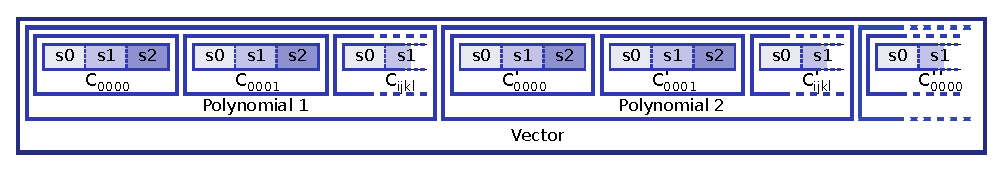
\includegraphics[scale=0.9]{memory_layout.eps} \\
    \vspace{0.5cm}
%    \hline

\includegraphics[scale=0.9]{memory_layout_gpu.eps} 
    \caption{Memory layout of a vector of polynomials with 192 bit integer coefficients.
             Each coefficient $\textsf{c}_{ijkl}$ consists of three 64 bit segments \textsf{s}.
             Top: Regular memory layout used on the CPU. Each coefficient is stored contiguously.
             Bottom: Memory layout used for intermediate results on the GPU. The coefficients are stored in an interleaved way grouping the segments according to their significance.
             Note that on the GPU we will have segments of only 32 bit width, which doubles the number of segments in return.
    }
    \label{fig:GPU_data_layout}
\end{figure}
This memory layout allows for a efficient coalesced access during the reduction at the end of the calculation.
Once the reduction is completed the result is transferred from the device memory back to the host using the regular memory layout.

Like for the SSE approach on the CPU our kernels on the GPU rely on 32 bit unsigned integer arithmetic.
However, on the GPU we were able to profit from hard-wired addition with carry \verb|addc.cc| and multiply-add with carry \verb|madc.cc| using NVIDIA parallel thread execution (PTX) inline assembly.
Contrary to the CPU where we used only schoolbook algorithms, we employ the Karatsuba algorithm \cite{Karatsuba1963} for the 256 bit integer multiplication on the GPU.
Even though the method does not require less operations than the schoolbook algorithm it is advantageous on the GPU, because it uses less multiplications and more additions on the 32 bit segments.
While on the CPU these operations are almost equally expensive, the addition on the NVIDIA Kepler has a 5 times higher throughput than the multiplication \cite{CUDAProgramming}.

% TODO write something on the number of threads used

%\begin{itemize}
%\item Many small tasks of the same form. $\rightarrow$ well suited for GPUs.
%\item {\bf Implementation details:}
%\item based on 32bit integers due to architecture.
%\item Element-wise polynomial multiplication + reduction at the end.
%\item Each thread calculates one coefficient $c_{IJKL}$ the product polynomial.
%\item Several coefficients $a_{ijkl}$, $b_{i'j'k'l'}$ of the polynomials to be multiplied contribute to the same coefficient $c_{IJKL}$
%\begin{equation}
%    c_{IJKL} = \sum_{i,j,k,l} a_{ijkl} \cdot b_{I-i,J-j,K-k,L-l}
%\end{equation}
%\item The number of terms in this sum depends on the orders $I,J,K,L$ of the resulting coefficient $\rightarrow$ load in-balance
%\item {\color{blue} We design an execution plan. We group the coefficients of a fictive result polynomial by packet of 32 } into a task and distribute them among the warps of threads (Fig.\ \ref{fig:GPU_load_balance}).
%\item Since threads within a warp are executed in a lockstep manner, we try to give all threads within a warp the same amount of work. This way the threads have to wait as little as possible for the other threads of the warp to finish.
%\item We group the coefficients by 32 into a ``task'' and distribute them among the warps of threads (Fig.\ \ref{fig:GPU_load_balance}), i.e.\ each thread calculates one coefficient of the resulting polynomial.
%\item Each thread of the warp gets the indices of the resulting coefficient and determines the necessary terms to calculate the output coefficient.
%\item Reduction is implemented according to the best practices by NVIDIA (TODO reference)
%%\item {\color{blue} This algorithm is efficient whatever the type of polynomial. But the termination of the contributions of an output coefficient can be tricky}
%\item We use the Karatsuba algorithm \cite{Karatsuba1963} for the largest extended multiplication (256 bit to 512 bit) on GPU, because an integer addition requires substantially less cycles than multiplication the GPU.
%\item Using NVIDIA parallel thread execution (PTX) assembly language to benefit from hardware carry bit propagation \verb|addc.cc| and multiply-add with carry bit propagation \verb|madc.cc|.
%\end{itemize}
%%%%%%%%%%%%%%%%%%%%%%%%%%%%%%%%%%%%%%%%%%%%%%%%%%%%%%%%%%%%%%%%%%%%%%%%%%%%%%%

\section{Benchmarks}
\paragraph{Simple integer operations}
We benchmarked the large integer part of the library on an Intel Sandy bridge Xeon E5-2670 node with 32 logical cores
and compared against the commonly used GNU Multiple Precision Arithemtic library (GMP).
The results are shown in table \ref{tab:vli_vs_gmp}.
\begin{table}
   \centering
   \begin{tabular}{l|cc|r}
    Operation & Execution & time [s] & Speed-up\\
      & GMP & VLI & \\
    \hline
   \verb|add|, 128 bit & 1.11 & 0.28 & {\bf 3.96x} \\
   \verb|add|, 192 bit & 1.21 & 0.42 & 2.88x \\
   \verb|add|, 256 bit & 1.11 & 0.77 & 1.44x \\
   \verb|add|, 320 bit & 1.25 & 0.94 & 1.32x \\
   \verb|add|, 384 bit & 1.25 & 0.91 & 1.37x \\
   \verb|add|, 448 bit & 1.34 & 0.97 & 1.38x \\
   \verb|add|, 512 bit & 1.31 & 1.04 & {\bf 1.26x} \\
   \hline
   \verb|mul|, 128 bit $\rightarrow$ 256 bit & 1.36 & 0.93 & 1.46x \\
   \verb|mul|, 192 bit $\rightarrow$ 384 bit & 3.21 & 1.18 & {\bf 2.72x} \\
   \verb|mul|, 256 bit $\rightarrow$ 512 bit & 3.74 & 2.04 & 1.83x \\ 
   \end{tabular}
   \caption{Execution time comparison of simple integer operations using the GNU Multiprecision Library and the VLI library for $10^8$ operations.}
   \label{tab:vli_vs_gmp}
\end{table}
Comparing the execution time of simple addition and multiplication operations our implementation for fixed size integers is between $26\%$ and $296\%$ faster for the addition and up to $172\%$ faster for the multiplication.
Note that the reported time is the pure execution time of the operation. All variables were allocated before.
The allocation will 
Since our integer library is stack based we do not need expensive calls to \verb|malloc| like GMP, which will give an additional speedup for the inner product, where multiple allocations are necessary.

%\begin{itemize}
%\item pure CPU benchmarks were done on a Sandy bridge Intel Xeon E5-2670 with 32 logical cores.
%\item Comparing the execution time of simple addition and multiplication operations our implementation for fixed size integers is between $26\%$ and $296\%$ faster for the addition and up to $172\%$ faster for the multiplication (table \ref{tab:vli_vs_gmp}).
%\item Note that the reported time is the pure execution time of the operation. All variables were allocated before.
%Since our integer library is stack based we do not need expensive calls to \verb|malloc|, which will give an additional speedup for the inner product.
%\end{itemize}

\paragraph{Optimized inner product with GPU accelerator}
The benchmarks for the inner product were again performed on the Intel Sandy bridge node for the pure CPU version of the inner product.
The GPU benchmarks were performed on Todi, a Cray XK7 with NVIDIA Tesla K20X GPUs and AMD Opteron CPUs, at the Swiss Center for Scientific Computing (CSCS).
The test cases are inner products of two vectors of dimension 4096 with ``dense'' and ``triangular'' polynomials of order 1 to 14 with 128 and 256 bit integer coefficients.
Since the inner product will double the order of the polynomial and the width of the large integer coefficients, the test cases will result in polynomials of order 2 to 28 with 256 and 512 bit integer coefficients, respectively.

Figure \ref{fig:performance_large_int_ops} shows the performance of the inner product for the various test cases in number of large integer operations per second.
Monovariant polynomials show a rather poor performance of at most $1.6 \text{G large integer OP/s}$ on the CPU.


\begin{itemize}
%\item GPU benchmarks were performed on Todi, a Cray XK7 with NVIDIA Tesla K20X GPUs and AMD Opteron CPUs, at the Swiss Center for Scientific Computing (CSCS)
%\item Testcase: inner product of two vectors dimension 4096, with ``dense'' and
%``triangular'' polynomials of order 1 to 14 with 128 and 256 bit integer
%coefficients. Which will result in polynomials of order 2 to 28 with 256 and 512 bit integer coefficients, respectively.
\item We estimate the performance in integer operations per second (IOP/s).
\item For the GPU performance estimate we only consider the instructions for the polynomial-polynomial multiplications and neglect the reduction at the end of the inner product.
\begin{figure}[t!]
    \centering
    \mbox{
        \hspace{-0.5cm}
        \includegraphics[scale=0.37, angle=-90]{ME128.eps} 
        \hspace{-0.4cm}
        \includegraphics[scale=0.37, angle=-90]{MC128.eps} 
    }
    \caption{Comparison of the inner product with and without GPU accelerator. Left: Inner product of dense polynomials with up to 3 variables and 126 to 256 bits coefficients. Right: Inner product of triangular polynomials with up to 3 variables and 126 to 256 bits coefficients. Size of the vector 4096. GMP gives similar results independent of the polynomial structure.}
    \label{fig:performance_large_int_ops}
\end{figure}

\begin{figure}[t!]
    \centering
    \mbox{
        \hspace{-0.5cm}
        \includegraphics[scale=0.37, angle=-90]{ME128MIPS.eps} 
        \hspace{-0.4cm}
        \includegraphics[scale=0.37, angle=-90]{MC128MIPS.eps} 
        %\hspace{-0.4cm}
        %\includegraphics[scale=0.25, angle=-90]{ME256.eps} 
    }
    \caption{Performance of the inner product of two vectors of dimension 4096 with ``dense'' (left) and ``triangular'' (right) polynomials having 128 bit coefficients on a NVIDIA Tesla K20X (GK110).}
    \label{fig:ResMEMIPS}
\end{figure}  
\item We reach up to $214$ GIOP/s using 32 bit multiply-add (\verb|madc|)
\item Theoretical maximum for the NVIDIA Tesla K20X is given by Number of Multiprocessors (SMX) $\cdot$ Clock frequency $\cdot$ Instruction throughput of \verb|madc|  =  $14 \, \mathrm{SMX} \cdot 732 \, \mathrm{MHz} \cdot 32 \, \mathrm{ IOP / cycle / SMX} = 327 \, \mathrm{GIOP/s}$. (Multiply-add throughput taken from \cite{CUDAProgramming}).
\item We reach $65\%$ of the peak.
\item Poor performance for low orders as well as for polynomials in 1 symbolic variable, since too little coefficients need to be calculated to saturate the number of available threads (Fig. \ref{fig:ResMEMIPS}).
\item Maximal performance for ``dense'' polynomial in 3 variables with a truncation at 7th order, where we employ $(2\cdot7+1)^3 = 3375$ threads. Using more threads may yield an even better performance, but we start to exceed the size of the texture memory cache and have to load data from the device memory more often, which causes the decrease of performance for higher orders.
\item Polynomials in 4 symbolic variables only up to 6th order due to memory limitations on the device. Could be overcome by splitting the vectors and performing the inner product on these parts sequentially.
\item Performance for ``triangular'' polynomials rises lower with increasing order, because the number of threads used grows slower with the order than for ``dense'' polynomials.
\end{itemize}

%%%%%%%%%%%%%%%%%%%%%%%%%%%%%%%%%%%%%%%%%%%%%%%%%%%%%%%%%%%%%%%%%%%%%%%%%%%%%%%

\section{Conclusion}
\begin{itemize}
\item TODO
\item Extend integers up to 2048 bits.
\item Allow more polynomial structures
\item License?
\end{itemize}

%%%%%%%%%%%%%%%%%%%%%%%%%%%%%%%%%%%%%%%%%%%%%%%%%%%%%%%%%%%%%%%%%%%%%%%%%%%%%%%
\bibliographystyle{llncs2e/splncs}
\bibliography{biblio/vlibib}

\end{document}
